\documentclass [11pt,a4paper,dvipdfmx]{ujarticle}
%
\usepackage{amsmath,amssymb}
\usepackage{bm}
\usepackage{graphicx}
\usepackage{ascmac}
\usepackage{booktabs}
\usepackage{enumitem}

\usepackage[
  a4paper,
  top=30mm,
  bottom=30mm,
  left=25mm,
  right=25mm
]{geometry}
%

\DeclareMathOperator{\divergence}{div} % ダイバージェンス
\DeclareMathOperator{\grad}{grad}     % グラディエント
\DeclareMathOperator{\rot}{rot}       % ローテーション
%

\title{プログラミング演習(C/C++) 中間レポート}
\author{23K0043 村上実優}
\date{\today}

\begin{document}
\maketitle
\newpage
\section*{実行環境}
この課題に取り組むときの実行環境について以下に示す。
\begin{itemize}
  \item \textbf{機種} MacBook Air(M1, 2020) ,  Apple M1チップ , 8GB
  \item \textbf{OS} MacOS Sequoia 15.5
  \item \textbf{コンパイラ} Apple clang version 17.0.0
\end{itemize}
\section{目的}
以下の基本的な処理の性能を各設問の方法で調査し、その性能差について考察・議論する。
\begin{enumerate}
  \item int変数と定数の加算
  \item int変数同士の加算
  \item long long 変数と定数の加算
  \item long long 変数同士の加算
  \item float 変数と定数の加算
  \item float 変数同士の加算
  \item double 変数と定数の加算
  \item double 変数同士の加算
\end{enumerate}

\section{背景}
次に示す方法で処理を行ったものを、処理一回あたりの実行時間(μs)で比較することで、どのような処理が実行時間が長く重い処理なのかを議論・考察する。
\clearpage
\section{実行結果}
\subsection{eval1-1}
目的で述べた1$\sim$8の処理を行うプログラムを作成して実行時間の計測と出力を行った。

loopは100000000回と設定し、for文中の処理も含めると400000000回の計算を行った時の実行時間を計測した。
また、1つの処理に対して10回試行を行い、その平均値を処理の実行時間とみなした。

実行時間をまとめたものが以下の表1である。
\begin{table}[htbp]
  \centering
  \caption{eval1-1 実行時間の測定結果}
  \label{tab:eval1-1-results}
  \begin{tabular}{ccrr}
    \toprule
    ID & データ数 & 平均実行時間 (μs) & 標準偏差 (μs) \\
    \midrule
    1 & 10 & 97953.70 & 6784.34 \\
    2 & 10 & 130289.00 & 1651.98 \\
    3 & 10 & 115265.40 & 1321.43 \\
    4 & 10 & 130149.20 & 1167.31 \\
    5 & 10 & 98956.10 & 935.59 \\
    6 & 10 & 126676.80 & 836.78 \\
    7 & 10 & 98573.10 & 685.51 \\
    8 & 10 & 128478.60 & 975.39 \\
    \bottomrule
  \end{tabular}
\end{table}

また、この結果を以下の図1にまとめた。
\begin{figure}[htbp]
  \centering
  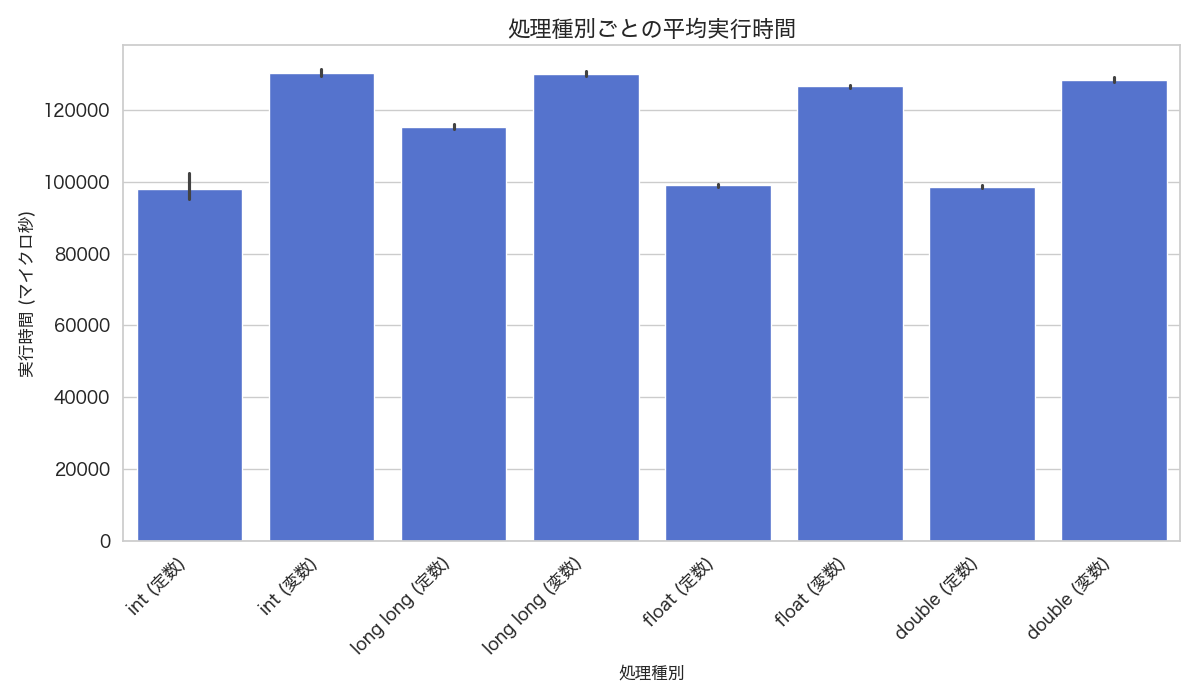
\includegraphics[width=0.8\linewidth]{result1-1.png}
  \caption{eval1-1 実行時間の測定結果}
\end{figure}

棒グラフの黒い棒線は信頼区間を示している。
\clearpage
\subsection{eval1-2}
目的で述べた1$\sim$8の各変数を大きな配列に確保し、処理を行うプログラムを作成して実行時間の計測と出力を行った。

loopは390625回と設定し、for文中の処理も含めると400000000回の計算を行った時の実行時間を計測した。
また、1つの処理に対して10回試行を行い、その平均値を処理の実行時間とみなした。

実行時間をまとめたものが以下の表2である。
\begin{table}[htbp]
  \centering
  \caption{eval1-2 実行時間の測定結果}
  \label{tab:eval1-2-results-final}
  \begin{tabular}{ccrr}
    \toprule
    ID & データ数 & 平均実行時間 (μs) & 標準偏差 (μs) \\
    \midrule
    1 & 10 & 224679.60 & 216.51 \\
    2 & 10 & 276329.10 & 168.17 \\
    3 & 10 & 226661.60 & 211.33 \\
    4 & 10 & 277714.20 & 139.73 \\
    5 & 10 & 226027.00 & 227.14 \\
    6 & 10 & 277799.40 & 385.66 \\
    7 & 10 & 230193.00 & 122.99 \\
    8 & 10 & 278635.00 & 143.76 \\
    \bottomrule
  \end{tabular}
\end{table}

また、この結果を以下の図2にまとめた。
\begin{figure}[htbp]
  \centering
  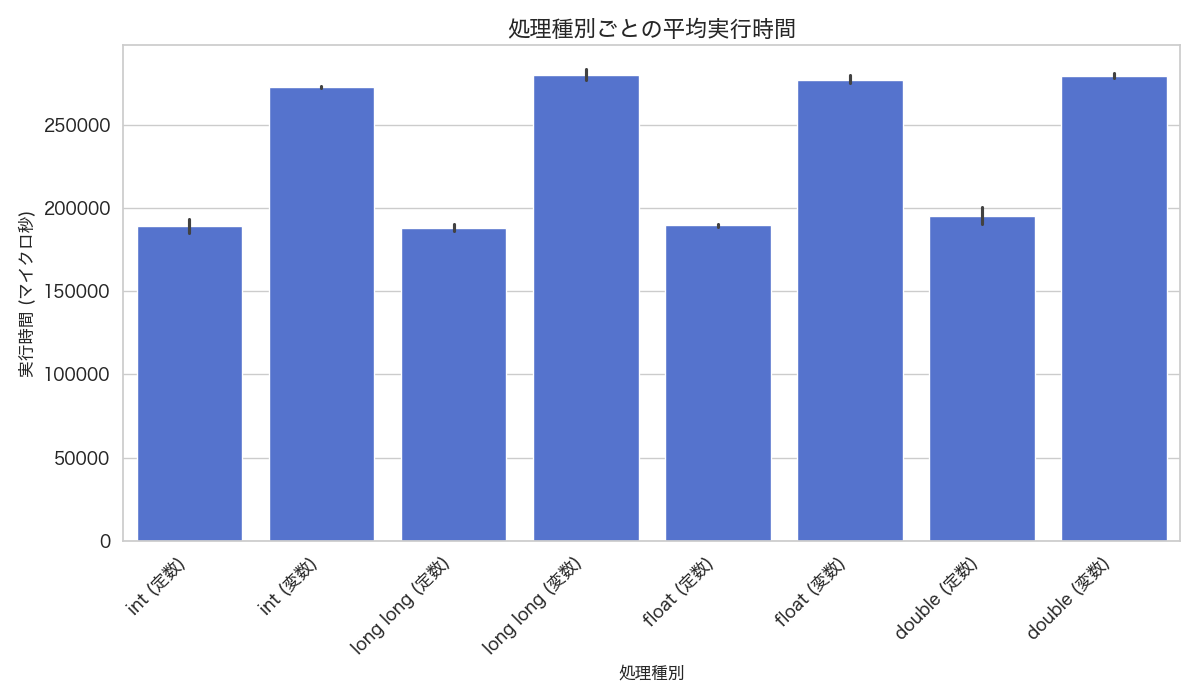
\includegraphics[width=0.8\linewidth]{result1-2.png}
  \caption{eval1-2 実行時間の測定結果}
\end{figure}

棒グラフの黒い棒線は信頼区間を示している。
\clearpage
\section{考察}
以上の結果からそれぞれの実行結果について考察を行う。
\subsection{eval1-1}
変数同士の加算に比べて、変数と定数の加算を行っているものの方がかなり実行時間が短くなっている。これは定数はメモリアクセスを必要としない即値であったため、実行時間に差が出たのだと考える。

また、long long変数と定数の加算のみ、他の変数と定数の加算よりも実行時間が長くなっている。原因として、変数のbit数に着目したが、同様に64bitの変数であるdouble型はそうではなかったのでなぜ実行時間が長くなったのか判明することはできなかった。
\subsection{eval1-2}
こちらも変数同士の加算に比べて、変数と定数の加算を行っているものの方がかなり実行時間が短くなっている。これも定数はメモリアクセスを必要としない即値であったため、実行時間に差が出たのだと考える。

そして、こちらはlong long変数と定数の加算のみ、他の変数と定数の加算よりも実行時間が長くなることはなかった。これは、eval1-1の計算よりもはるかに時間がかかる計算をeval1-2は行っているため、差が出にくくなったのではないかと考える。
\subsection{2つのプログラムの比較}
これら2つのプログラムの結果を比べると、同じ実行回数に対して圧倒的にeval1-2の操作の方が実行時間が長くなっていることがわかる。つまり、スカラー計算を行うよりも、配列の計算を行う方が実行時間が長くなるということが分かる。
これはスカラー計算はレジスタに値を保持していることができるが、配列計算はそれぞれの配列までデータを探しに行った上で計算を行うという段階を踏まないといけないので、メモリアクセスの時間などで実行時間が長くなってしまうのだと考える。
\clearpage
\section{任意課題}
この課題ではeval1-1の5で行ったfloat変数と定数の加算について、定数の型を変更して比較を行う。詳しい比較内容は以下に示す。
\begin{enumerate}[start = 9]
  \item 定数に整数を使う
  \item 定数に小数表現を使う
  \item 定数をfloat()で囲う
\end{enumerate}
\section{実行結果}
任意課題で述べた9$\sim$11の処理を行うプログラムをeval1-3として作成して実行時間の計測と出力を行った。

loopは100000000回と設定し、for文中の処理も含めると400000000回の計算を行った時の実行時間を計測した。
また、1つの処理に対して10回試行を行い、その平均値を処理の実行時間とみなした。

実行時間をまとめたものが以下の表3である。
\begin{table}[htbp]
  \centering
  \caption{eval1-3 実行時間の測定結果}
  \label{tab:eval1-3-results-id}
  \begin{tabular}{ccrr}
    \toprule
    ID & データ数 & 平均実行時間 (μs) & 標準偏差 (μs) \\
    \midrule
    9  & 10 & 101788.50 & 3361.30 \\
    10 & 10 & 126837.10 & 777.59 \\
    11 & 10 & 99436.50 & 883.59 \\
    \bottomrule
  \end{tabular}
\end{table}

また、この結果を以下の図3にまとめた。
\begin{figure}[htbp]
  \centering
  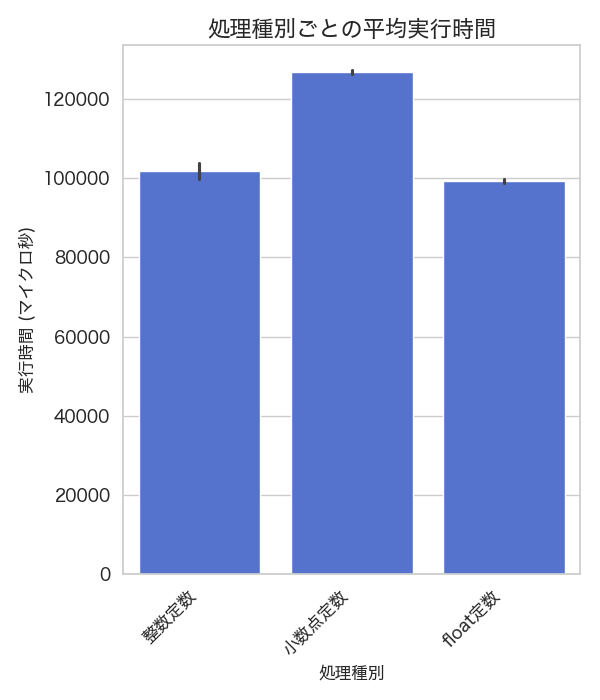
\includegraphics[width=0.4\linewidth]{result1-3.png}
  \caption{eval1-3 実行時間の測定結果}
\end{figure}

棒グラフの黒い棒線は信頼区間を示している。
\clearpage
\section{考察}
以上の結果より、小数表現の定数の時のみ実行時間が長くなっている。これはc++では、2.0のように書かれた数はdouble型として捉えるため、他の2つの定数よりも型変換を行う回数が増え、実行時間が長くなるのではないかと考える。

\section{結論}
このレポートでは8種の基本的な加算処理について、スカラー計算と配列計算の2つの手法で性能測定を行い、比較と考察を行った。

この結果、メモリアクセスが必要になる変数同士の加算は即値である定数を使用できる変数と定数の加算よりも実行時間が長いことが確認できた。
また、総演算回数が一緒である場合、レジスタに値を保持できるスカラー計算よりも、メモリアクセスを必要とする配列計算の方が実行時間が長いことが確認できた。

また、任意課題ではfloat型と3種の定数との加算処理についてスカラー計算を行い、性能測定を行った。

この結果、少数表現の定数のみdouble型として扱われるため、型変換が行われる回数が増え、実行時間が長くなることが確認できた。


\end{document}